\documentclass{scrartcl}

\usepackage[linear]{handout}
\usepackage{bbm}
\usepackage{siunitx}
\usepackage{circuitikz}
% \usepackage{mlmodern}
% \usepackage{gfsartemisia}
\ihead{\sffamily\bfseries\footnotesize{Experiment 05}}
\ohead{\sffamily\footnotesize\textbf{}} 

\title{
        \Large\textsc{PH3204: Electronics Lab} \\
        \vspace{10pt}
        % \Large\textsc{Experiment 02} \\
        % \vspace{0.1cm}
        \Huge \textbf{Study of a 555 timer IC} \\
}

% \subtitle{}

\author{Sabarno Saha \\ \texttt{22MS037} \\ Grp. B-10}

\date{\normalsize
        \textit{Indian Institute of Science Education and Research, Kolkata, \\
        Mohanpur, West Bengal, 741246, India.}
        % \vspace{10pt}
        % \today
}
\newcommand{\1}{\mathbbm{1}}
\newcommand{\ichi}{\tilde{\chi}}
\newcommand{\irho}{\tilde{\rho}}
\newcommand{\ihsr}{\tilde{H}_{SR}}
\newcommand{\G}{\Gamma}
\newcommand{\iG}{\tilde{\Gamma}}
\newcommand{\is}{\tilde{s}}
\newcommand{\h}{\mathbb{H}}
\newcommand{\nbar}{\bar{n}}

\graphicspath{{./code/}}

\begin{document}
\maketitle
\tableofcontents

\section{Aim}
To study the use of a 555 timer as an astable multivibrator and to determine the time period of the output waveform.\\.

\section{Theory}
In this experiment, we will be using a 555 timer to make an astable multivibrator. An astable 
multivibrator is a circuit that continuously switches between its two unstable states, producing a square wave output. 
The 555 timer is a versatile integrated circuit that can be used in various configurations, including monostable and astable modes.
The 555 timer consists of two voltage comparators, a flip-flop, a discharge transistor, and a resistor divider network. 
In astable mode, the timer oscillates between its high and low states, generating a square wave output. 
The frequency and duty cycle of the output waveform can be controlled by adjusting the values of external resistors and
 capacitors connected to the timer. We will also study these properties in this experiment.
\section{Circuit Diagram}
\tikzstyle{icdev}=[draw, text width=5.5em, minimum height=7.3em]
\begin{figure}[H]
    \centering
    \begin{tikzpicture}[every node/.style = {font = \tiny},american]
        \draw (0,4) node[left]{$\mathrm{V_{s}}$}  % from top Vcc to bottom Gnd
            to[short,o-] (0.8,4)
            to[/tikz/circuitikz/bipoles/length=0.7cm,R, l_=$\mathrm{R_1}$] (0.8,2.6) % set bipole device size
            to[/tikz/circuitikz/bipoles/length=0.7cm,R, l_=$\mathrm{R_2}$] (0.8,1.8)  to[/tikz/circuitikz/bipoles/length=0.7cm,C, l_=$\mathrm{C_1}$] (0.8,0.09) -- (0.8,0)
            to[short,-o] (0,0) node[left]{GND}
        ;
        \node (digichip) [icdev,xshift=3cm,yshift=2cm] {};
        \draw[blue] (3,2) node [align=center]{};  % position IC device body
    % top terminal lines/pins - 4 RESET, 8 Vcc
        \path [draw](0.8,4) -| (2.5,3.4) node[below]{RESET} node[above left]{4};
        \path [draw](2.5,4) -| (3.5,3.4) node[below]{$\mathrm{V_{cc}}$} node[above left] {8};
    % bottom terminal lines/pins - 1 GND, 5 CTRL
        \path [draw](0.8,0) -| (2.5,0.6) node[above]{GND} node[below left]{1};
        \path [draw](2.5,0) -- (3.5,0)
            to[/tikz/circuitikz/bipoles/length=0.7cm,C](3.5,0.6)  
            node[above]{CTRL} node[below right]{\ \ 5}; % C = 10nf
    % leftside terminal lines/pins - 7 DIS, 6 THR, 2 TRG
        \draw (0.8,2.7) -- (1.83,2.7) node[right]{DIS} node[above left]{7}
             (1.83,2) node[right]{THR} node[above left]{6} |- (1.3,2) -- (1.3,1.5) --
            (0.8,1.5) -- (1.83,1.5) node[right]{TRG} node[above left]{2};
    % rightside terminal line/pin - 3 out
        \draw (4.17,2) node[left]{OUT} -- (4.8,2) node[above left]{3} to[short,o-] (4.8,2);
    \end{tikzpicture}
    \caption{Circuit Diagram of 555 Timer IC}
    \label{fig:555}
\end{figure}
The pins of the 555 timer are as follows:
\begin{itemize}
    \item Pin 1: Ground (GND): This pin is connected to the ground of the circuit.
    \item Pin 2: Trigger (TRIG) - This pin is used to trigger the timer.
    \item Pin 3: Output (OUT) - This pin provides the output of the timer. 
    \item Pin 4: Reset (RESET) - This pin is used to reset the timer. A low signal on this pin resets the flip-flop, causing the output to go low.
    \item Pin 5: Control Voltage (CTRL) - This pin is used to control the timing of the timer, by changing the threshold voltage usually set at $2V_{cc}/3$. It is usually connected to a capacitor to filter noise.
    \item Pin 6: Threshold (THR) - This pin is used to monitor the voltage across the timing capacitor. When this voltage exceeds 2/3 of the supply voltage, the flip-flop is reset.
    \item Pin 7: Discharge (DISCH) - This pin is used to discharge the timing capacitor. When the flip-flop is reset, this pin is connected to ground, allowing the capacitor to discharge.
    \item Pin 8: Supply Voltage (VCC) - This pin is connected to the positive supply voltage.
\end{itemize} 

The input and output waveforms of the 555 timer in astable mode are shown below. 
\begin{figure}[H]
    \centering
    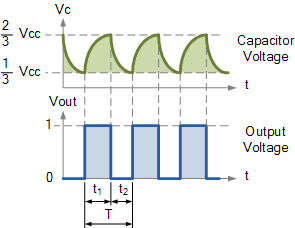
\includegraphics[width=0.3\textwidth]{waveforms.png}
    \caption{Input and Output Waveforms of 555 Timer in Astable Mode.  (Source: The Internet)}
    \label{fig:waveform}
\end{figure}

The frequency of the output waveform can be altered by changing the values of the resistors and capacitors connected to the timer.
The frequency of the output waveform is given by the formula:
\begin{equation}
    f = \frac{1}{\ln(2)(R_1 + 2R_2)C_1}
\end{equation}
The uptime and downtime of the output waveform can be calculated using the following formulae:
\begin{align}
    T_{H} = \ln(2)(R_1 + R_2)C_1\quad\quad;\quad\quad
    T_{L} = \ln(2)R_2C_1
\end{align}
The duty cycle(D) is defined as the time the output is high divided by the total time period of the output waveform.
The duty cycle, expressed as a percentage, can be calculated using the formula:
\begin{equation}
    D = \frac{T_{H}}{T_{H} + T_{L}} \times 100 = \frac{R_1 + R_2}{R_1 + 2R_2} \times 100 
\end{equation}

\section{Data}

The following data was obtained from the experiment. We calculate the up and down times using the oscilloscope.

\begin{table}[H]
    \centering
    \begin{tabular}{|l|l|l|l|l|l|l|l|r|}
    \hline
        \textbf{\small C($\mu F$)} & \textbf{\small$R_1$($\Omega$)} & \textbf{\small$R_2$($\Omega$)} & \textbf{\small$f_T$(Hz)} & \textbf{$T_H$ (e) (s)} & \textbf{$T_L$(e)(s)} & \textbf{T(e)(s)} & \textbf{$f_{e}$(Hz)} & \textbf{Err(\%)} \\ \hline
        0.001 & \num{E+03} & \num{E+04} & \num{6.87E+04} & \num{7.2E-06} & \num{7.2E-06} & \num{1.44E-05} & \num{6.94E+04}  & \num{1.08 }\\ 
        0.001 & \num{E+04} & \num{E+05} & \num{6.87E+03} & \num{7.4E-05} & \num{6.6E-05} & \num{1.40E-04} & \num{7.14E+03}  & \num{3.97 }\\ 
        0.001 & \num{E+05} & \num{E+06} & \num{6.87E+02} & \num{7.3E-04} & \num{6.7E-04} & \num{1.40E-03} & \num{7.14E+02}  & \num{3.97 }\\ \hline
        0.01  & \num{E+03} & \num{E+04} & \num{6.87E+03} & \num{8.4E-05} & \num{7.6E-05} & \num{1.60E-04} & \num{6.25E+03}  & \num{9.02 }\\ 
        0.01  & \num{E+04} & \num{E+05} & \num{6.87E+02} & \num{8.7E-04} & \num{7.9E-04} & \num{1.66E-03} & \num{6.02E+02}  & \num{12.31} \\
        0.01  & \num{E+05} & \num{E+06} & \num{6.87E+01} & \num{7.8E-03} & \num{8.1E-03} & \num{1.59E-02} & \num{6.29E+01}  & \num{8.45 }\\ \hline
        0.1   & \num{E+03} & \num{E+04} & \num{6.87E+02} & \num{4.4E-04} & \num{4.2E-04} & \num{8.60E-04} & \num{1.16E+03}  & \num{69.26} \\
        0.1   & \num{E+04} & \num{E+05} & \num{6.87E+01} & \num{4.8E-03} & \num{4.8E-03} & \num{9.60E-03} & \num{1.04E+02}  & \num{51.63} \\ 
        0.1   & \num{E+05} & \num{E+06} & \num{6.87E+00} & \num{5.0E-02} & \num{4.8E-02} & \num{9.80E-02} & \num{1.02E+01}  & \num{48.53} \\\hline
        1     & \num{E+03} & \num{E+04} & \num{6.87E+01} & \num{7.5E-03} & \num{7.0E-03} & \num{1.45E-02} & \num{6.90E+01}  & \num{0.39 }\\ 
        1     & \num{E+04} & \num{E+05} & \num{6.87E+00} & \num{7.7E-02} & \num{7.0E-02} & \num{1.47E-01} & \num{6.80E+00}  & \num{0.98 }\\ 
        1     & \num{E+05} & \num{E+06} & \num{6.87E-01} & \num{7.8E-01} & \num{7.0E-01} & \num{1.48E+00} & \num{6.76E-01}  & \num{1.65 }\\ \hline
        10    & \num{E+04} & \num{E+05} & \num{6.87E-01} & \num{7.9E-01} & \num{7.1E-01} & \num{1.50E+00} & \num{6.67E-01}  & \num{2.96 }\\ 
        10    & \num{E+05} & \num{E+06} & \num{6.87E-02} & \num{8.4}     & \num{6.9E+00} & \num{1.53E+01} & \num{6.54E-02}  & \num{4.86 }\\ 
        10    & \num{E+03} & \num{E+04} & \num{6.87E+00} & \num{7.8E-02} & \num{7.0E-02} & \num{1.48E-01} & \num{6.76E+00}  & \num{1.65 }\\ \hline
    \end{tabular}
    \caption{Data}
\end{table}
The following data was obtained from the experiment. We calculate the duty cycle using the oscilloscope.
\begin{table}[H]
    \centering
    \begin{tabular}{|l|l|l|l|l|}
    \hline
        \textbf{C ($\mu F$)} & \textbf{R1 (Ohm)} & \textbf{R2 (Ohm)} & \textbf{Expt. Duty Cycle(\%)} & \textbf{Theo. Duty Cycle(\%)}\\ \hline
        0.001 & \num{E+03} & \num{E+04}  & \num{5.00E-01} & \num{5.24E-01}            \\
        0.001 & \num{E+04} & \num{E+05}  & \num{5.29E-01} & \num{5.24E-01}            \\
        0.001 & \num{E+05} & \num{E+06}  & \num{5.21E-01} & \num{5.24E-01}            \\ \hline
        0.01  & \num{E+03} & \num{E+04}   & \num{5.25E-01} & \num{5.24E-01}           \\
        0.01  & \num{E+04} & \num{E+05}   & \num{5.24E-01} & \num{5.24E-01}           \\
        0.01  & \num{E+05} & \num{E+06}   & \num{4.91E-01} & \num{5.24E-01}           \\ \hline
        0.1   & \num{E+03} & \num{E+04}    & \num{5.12E-01} & \num{5.24E-01}          \\
        0.1   & \num{E+04} & \num{E+05}    & \num{5.00E-01} & \num{5.24E-01}          \\
        0.1   & \num{E+05} & \num{E+06}    & \num{5.10E-01} & \num{5.24E-01}          \\ \hline
        1     & \num{E+03} & \num{E+04}      & \num{5.17E-01} & \num{5.24E-01}        \\
        1     & \num{E+04} & \num{E+05}      & \num{5.24E-01} & \num{5.24E-01}        \\
        1     & \num{E+05} & \num{E+06}      & \num{5.27E-01} & \num{5.24E-01}        \\ \hline
        10    & \num{E+04} & \num{E+05}     & \num{5.27E-01} & \num{5.24E-01}         \\
        10    & \num{E+05} & \num{E+06}     & \num{5.49E-01} & \num{5.24E-01}         \\
        10    & \num{E+03} & \num{E+04}  & \num{5.27E-01} & \num{5.24E-01}      \\\hline
    \end{tabular}
    \caption{Duty Cycles}
\end{table}

\section{Observations}
We observe that the errors are quite small for most of the cases. The errors are less than 10\% for most of the cases.
The errors are quite large for the $1\mu F$ capacitor. We expect a linear fit between the experimental and theoretical frequencies.
The loglog plot is given below,
\begin{figure}[H]
    \centering
    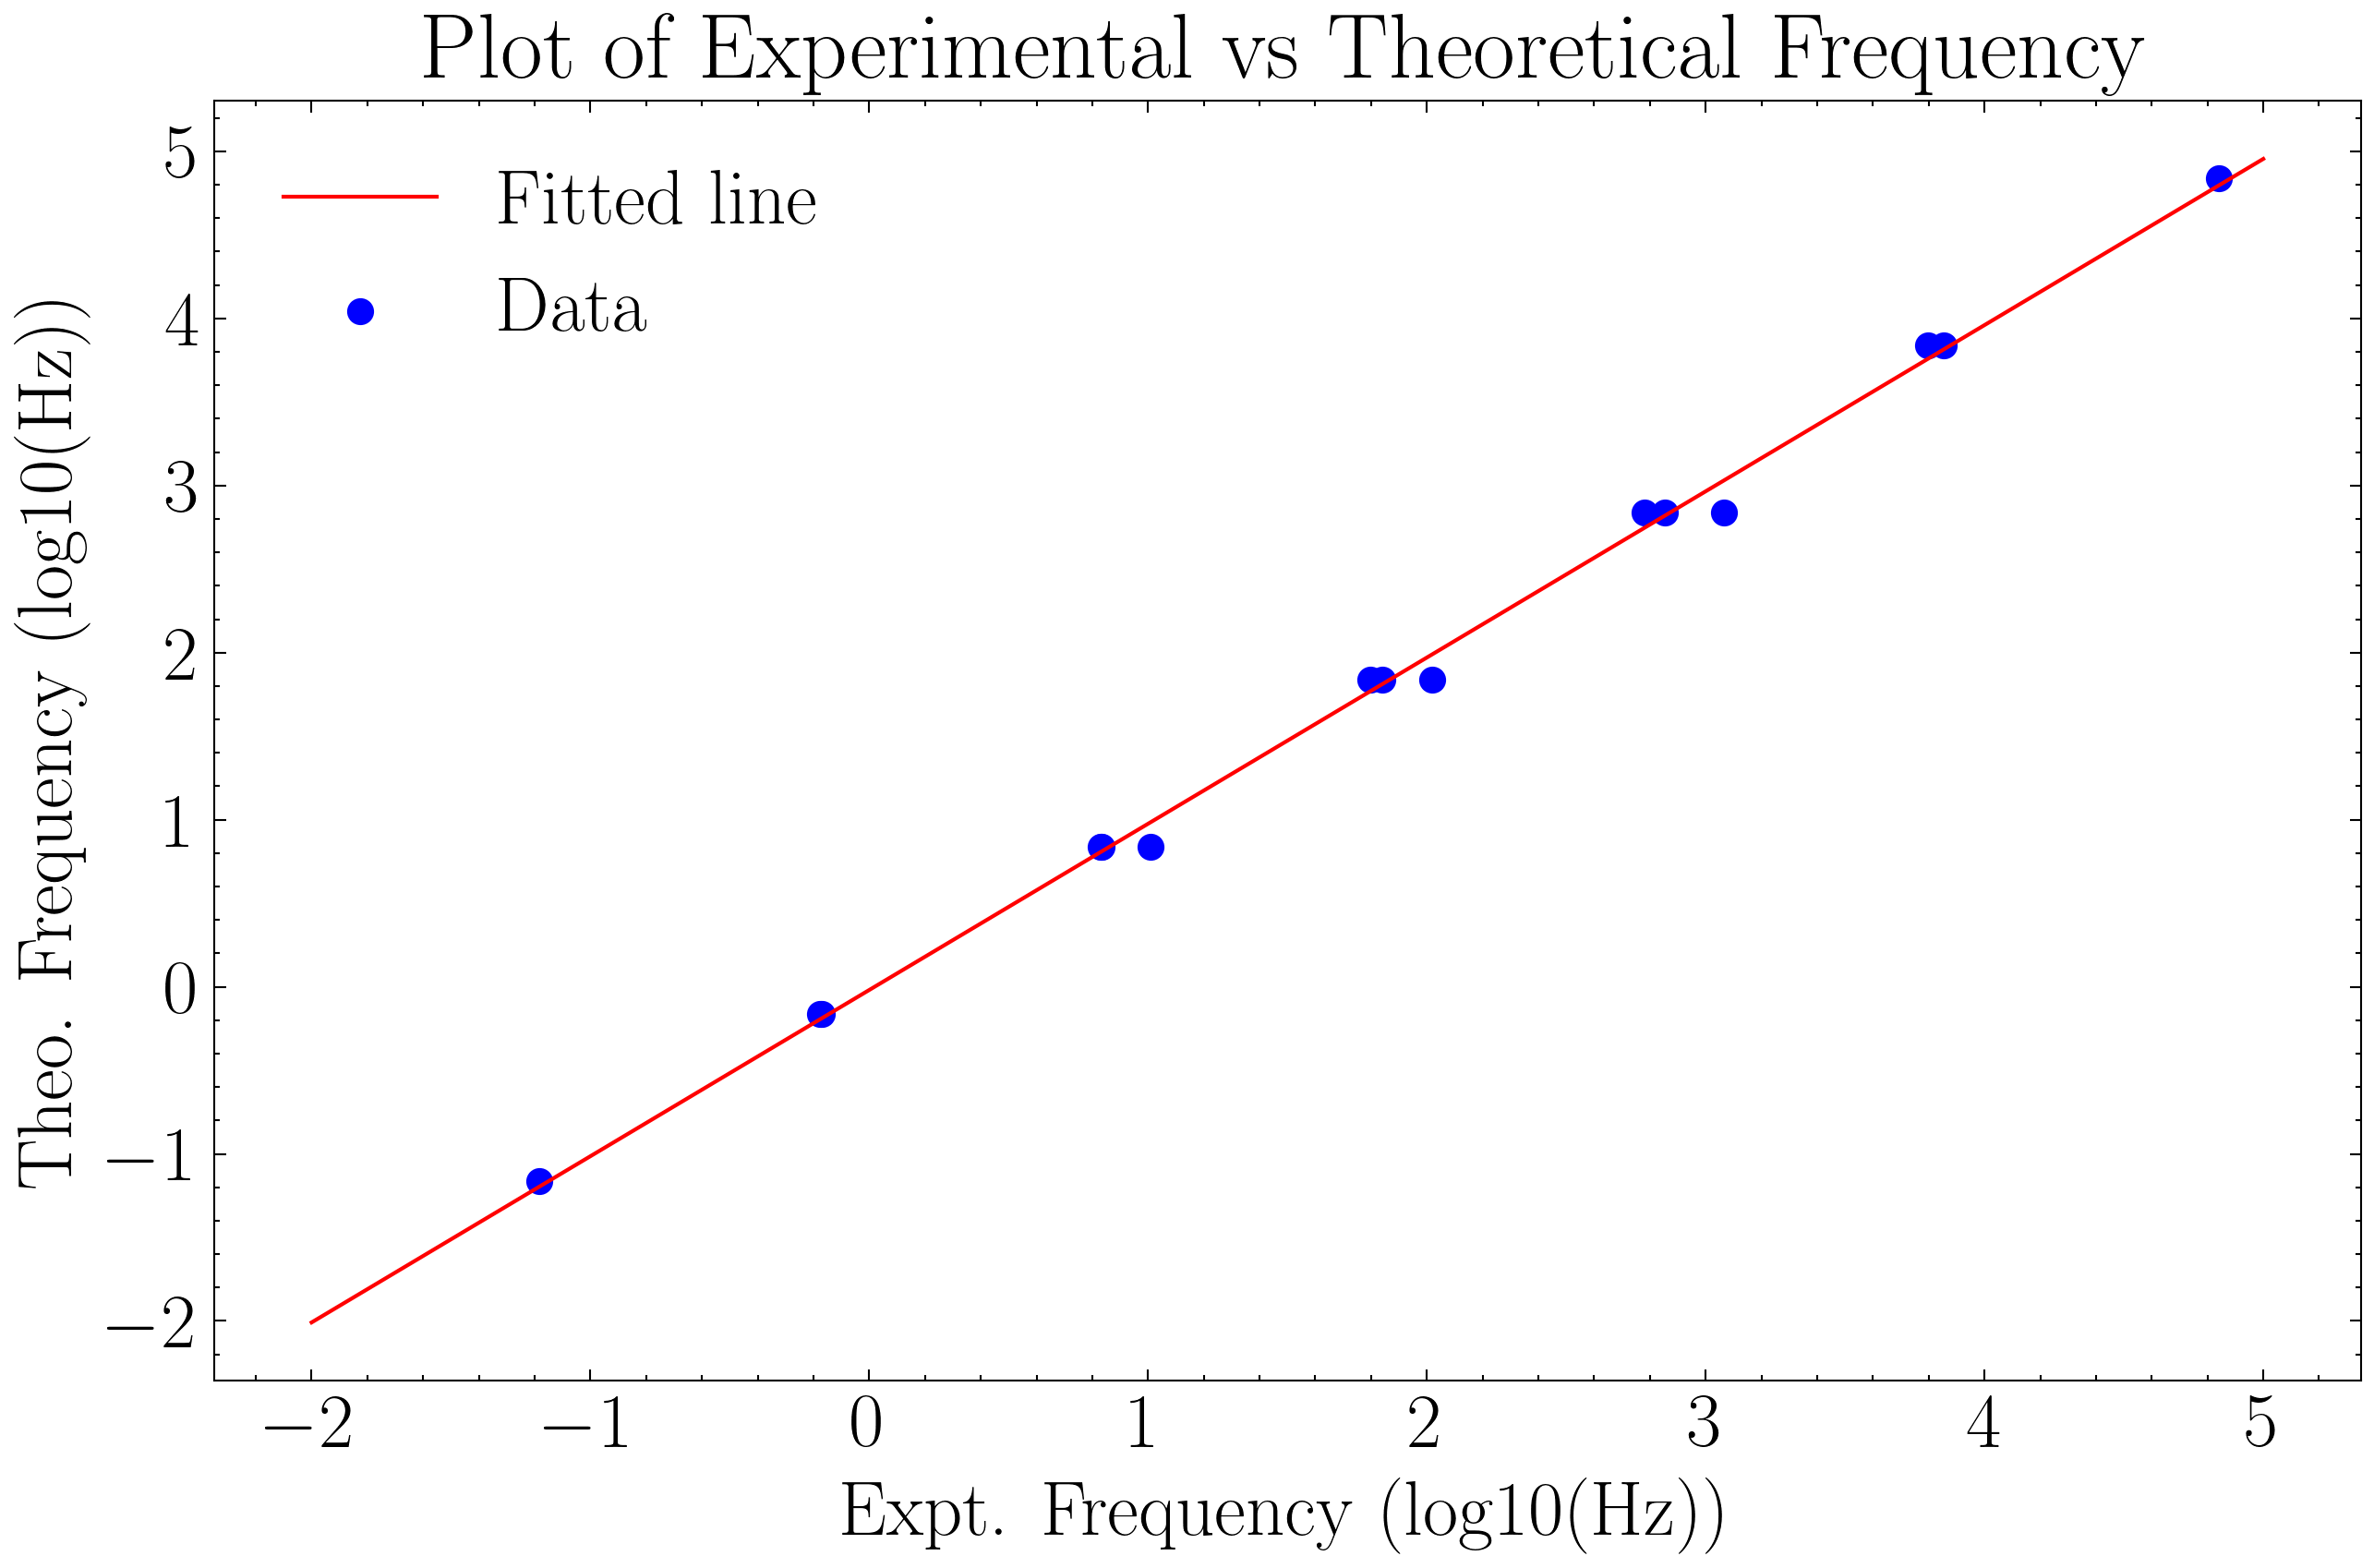
\includegraphics[width=0.8\textwidth]{expt_vs_theo.png}
    \caption{Loglog plot of the experimental and theoretical frequencies.}
    \label{fig:loglog}
\end{figure}


We expect a slope of 1. We obtain from the linear fit the slope to be $0.994 \pm 0.014$. We see that the
experiment matches the data quite well.

\section{Results}
The experiment demonstrated the use of a 555 timer to run a astable multivibrator. We were able to
calculate the frequency and duty cycle of the output waveform. The experimental values were in good agreement with the theoretical values.
The errors were less than 10\% for most of the cases. The errors were quite large for the $1\mu F$ capacitor.

\section{Error Analysis}
\begin{itemize}
        \item There are errors in the provided values of the resistors and capacitors. The resistors and capacitors are not ideal and have some tolerance.
        \item  The oscilloscope has some error in measuring the time period of the output waveform.
        \item The 555 timer is not ideal and can have internal variations in its characteristics.
        \item The power supply had some noise which can affect the output waveform.
        \item The breadboard connections can introduce errors to the output waveform.
\end{itemize}
\section{Conclusion}
We conclude the experiment by showing how the 555 timer can be used as an astable multivibrator. We were able to calculate the frequency and duty cycle of the output waveform. The experimental values were in good agreement with the theoretical values. 
\end{document}
%& \num{5.00E-01} & \num{5.24E-01}
%& \num{5.29E-01} & \num{5.24E-01}
%& \num{5.21E-01} & \num{5.24E-01}
%& \num{5.25E-01} & \num{5.24E-01}
%& \num{5.24E-01} & \num{5.24E-01}
%& \num{4.91E-01} & \num{5.24E-01}
%& \num{5.12E-01} & \num{5.24E-01}
%& \num{5.00E-01} & \num{5.24E-01}
%& \num{5.10E-01} & \num{5.24E-01}
%& \num{5.17E-01} & \num{5.24E-01}
%& \num{5.24E-01} & \num{5.24E-01}
%& \num{5.27E-01} & \num{5.24E-01}
%& \num{5.27E-01} & \num{5.24E-01}
%& \num{5.49E-01} & \num{5.24E-01}
%& \num{5.27E-01} & \num{5.24E-01}